\documentclass[table]{beamer}
%[]中可以使用draft、handout、screen、transparency、trancompress、compress等参数

%指定beamer的模式与主题
\mode<presentation>
{
  \usetheme{Madrid}
%\usetheme{Boadilla}
%\usecolortheme{default}
%\usecolortheme{orchid}
%\usecolortheme{whale}
%\usefonttheme{professionalfonts}
}

%\usetheme{Madrid}
%这里还可以选择别的主题:Bergen, Boadilla, Madrid, AnnArbor, CambridgeUS, Pittsburgh, Rochester, Warsaw, ...
%有导航栏的Antibes, JuanLesPins, Montpellier, ...
%有内容的Berkeley, PaloAlto, Goettingen, Marburg, Hannover, ...
%有最小导航栏的Berlin, Ilmenau, Dresden, Darmstadt, Frankfurt, Singapore, Szeged, ...
%有章和节表单的Copenhagen, Luebeck, Malmoe, Warsaw, ...

%\usecolortheme{default}
%设置内部颜色主题(这些主题一般改变block里的颜色);这个主题一般选择动物来命名
%这里还可以选择别的颜色主题,如默认的和有特别目的的颜色主题default,structure,sidebartab,全颜色主题albatross,beetle,crane,dove,fly,seagull,wolverine,beaver

%\usecolortheme{orchid}
%设置外部颜色主题(这些主题一般改变title里的颜色);这个主题一般选择植物来命名
%这里还可以选择别的颜色主题,如默认的和有特别目的的颜色主题lily,orchid,rose

%\usecolortheme{whale}
%设置字体主题;这个主题一般选择海洋动物来命名
%这里还可以选择别的颜色主题,如默认的和有特别目的的颜色主题whale,seahorse,dolphin

%\usefonttheme{professionalfonts}
%类似的还可以定义structurebold,structuresmallcapsserif,professionalfonts

% 控制 beamer 的风格,可以根据自己的爱好修改
%\usepackage{beamerthemesplit} %使用 split 风格
%\usepackage{beamerthemeshadow} %使用 shadow 风格
%\usepackage[width=2cm,dark,tab]{beamerthemesidebar}

%插入音标
%\usepackage{tipa}
%\AtBeginDocument{
  %\renewcommand\textipa{\fontencoding{T3}\selectfont}
%}
%\AtBeginDocument{
  %\renewcommand\textipa[2][r]{{\fontfamily{cm#1}\tipaencoding #2}}
%}
%\renewenvironment{IPA}[1][r]
 %{\fontfamily{cm#1}\tipaencoding}
 %{}

% 设定英文字体
%\usepackage{fontspec}
% Fix bugs for fontspec in TeXLive2015
\ifdefined\suppressfontnotfounderror
  \expandafter\let\csname xetex_suppressfontnotfounderror:D\endcsname
    \suppressfontnotfounderror
\else
  \expandafter\let\csname xetex_suppressfontnotfounderror:D\endcsname
    \luatexsuppressfontnotfounderror
\fi
\usepackage[no-math]{fontspec}
\setmainfont{Times New Roman}
\setsansfont{Arial}
\setmonofont{Courier New}

% 设定中文字体
\usepackage[BoldFont,SlantFont,CJKchecksingle,CJKnumber]{xeCJK}
%\setCJKmainfont[BoldFont={Adobe Heiti Std},ItalicFont={Adobe Kaiti Std}]{Adobe Song Std}
\setCJKmainfont[BoldFont={Adobe Heiti Std},ItalicFont={Adobe Kaiti Std}]{WenQuanYi Micro Hei}
\setCJKsansfont{Adobe Heiti Std}
\setCJKmonofont{Adobe Fangsong Std}
\punctstyle{hangmobanjiao}

\defaultfontfeatures{Mapping=tex-text}
\usepackage{xunicode}
\usepackage{xltxtra}

\XeTeXlinebreaklocale "zh"
\XeTeXlinebreakskip = 0pt plus 1pt minus 0.1pt

\usepackage{setspace}
\usepackage{colortbl,xcolor}
\usepackage{hyperref}
%\hypersetup{xetex,bookmarksnumbered=true,bookmarksopen=true,pdfborder=1,breaklinks,colorlinks,linkcolor=blue,filecolor=black,urlcolor=cyan,citecolor=green}
\hypersetup{xetex,bookmarksnumbered=true,bookmarksopen=true,pdfborder=1,breaklinks,colorlinks,linkcolor=cyan,filecolor=black,urlcolor=blue,citecolor=green}

% 插入图片
\usepackage{graphicx}
\graphicspath{{figures/}}
% 图文混排
%\usepackage{picins}
\usepackage{floatflt}

% 可能用到的包
\usepackage{amsmath,amssymb}
%插入多媒体
%\usepackage{media9}
%\usepackage{movie15}
\usepackage{multimedia}
\usepackage{multicol}
\usepackage{multirow}

% 定义一些自选的模板,包括背景、图标、导航条和页脚等,修改要慎重
% 设置背景渐变由10%的红变成10%的结构颜色
%\beamertemplateshadingbackground{red!10}{structure!10}
%\beamertemplatesolidbackgroundcolor{white!90!blue}
% 使所有隐藏的文本完全透明、动态,而且动态的范围很小
\beamertemplatetransparentcovereddynamic
% 使itemize环境中变成小球,这是一种视觉效果
\beamertemplateballitem
% 为所有已编号的部分设置一个章节目录,并且编号显示成小球
\beamertemplatenumberedballsectiontoc
% 将每一页的要素的要素名设成加粗字体
\beamertemplateboldpartpage

% item逐步显示时,使已经出现的item、正在显示的item、将要出现的item呈现不同颜色
\def\hilite<#1>{
 \temporal<#1>{\color{gray}}{\color{blue}}
    {\color{blue!25}}
}

\renewcommand{\today}{\number\year 年 \number\month 月 \number\day 日}

%五角星
\usepackage{MnSymbol}

%去除图表标题中的figure等
\usepackage{caption}
\captionsetup{labelformat=empty,labelsep=none}

\usepackage{tabu}
\usepackage{multirow}
%表格自动换行
\usepackage{tabularx} 

% 千分号
%\usepackage{textcomp}

%罗马数字
\makeatletter
\newcommand{\rmnum}[1]{\romannumeral #1}
\newcommand{\Rmnum}[1]{\expandafter\@slowromancap\romannumeral #1@}
\makeatother

%分栏
\usepackage{multicol}

%\usepackage{enumitem}
%\usepackage{enumerate}

%键盘
\usepackage{keystroke}

%心形
\usepackage{fdsymbol}

%插入源代码
\usepackage{listings}
\lstset{
  language=perl,                  % 程序语言名称:TeX, Perl, R, sh, bash, Awk
  basicstyle=\normalsize\tt,      %\tt指monospace字体族,程序源代码使用此族字体表示更加美观
  numbers=left,                   % 行号位置(左侧)
  numberstyle=\small,             % 行号字体的字号
  stepnumber=1,                   % 行号的显示步长
  numbersep=5pt,                  % 行号与代码间距
  backgroundcolor=\color{white},  % 背景色;需要 \usepackage{color}
  showspaces=false,               % 不显示空格
  showstringspaces=false,         % 不显示代码字符串中的空格标记
  showtabs=false,                 % 不显示 TAB
  tabsize=4, 
  frame=shadowbox,                % 把代码用带有阴影的框圈起来
  captionpos=b,                   % 标题位置
  breaklines=true,                % 对过长的代码自动断行
  breakatwhitespace=false,        % 断行只在空格处
  extendedchars=false,            % 解决代码跨页时,章节标题,页眉等汉字不显示的问题
  %escapeinside={\%*}{*},         % 跳脱字符,添加注释,暂时离开 listings 
  %escapeinside=``,
  commentstyle=\color{red!50!green!50!blue!50}\tt,  %浅灰色的注释
  rulesepcolor=\color{red!20!green!20!blue!20},     %代码块边框为淡青色
  keywordstyle=\color{blue!70}\bfseries\tt,         %代码关键字的颜色为蓝色,粗体
  identifierstyle=\tt,
  stringstyle=\tt,                % 代码字符串的特殊格式
  keepspaces=true,
  breakindent=1em,
  %breakindent=22pt,
  %breakindent=4em,
  breakautoindent=true,
  flexiblecolumns=true,
  aboveskip=1em,                  %代码块边框
  xleftmargin=2em,
  xrightmargin=2em
}

%\setbeamercolor{alerted text}{fg=magenta}
\setbeamercolor{bgcolor}{fg=yellow,bg=cyan}
%\setbeamercolor{itemize/enumerate body}{fg=green}

\begin{document}

%\includeonlyframes{current}

\logo{\includegraphics[height=0.08\textwidth]{tijmu.png}}

% 在每个Section前都会加入的Frame
\AtBeginSection[]
{
  \begin{frame}<beamer>
    %\frametitle{Outline}
    \frametitle{教学提纲}
    \setcounter{tocdepth}{3}
    \begin{multicols}{2}
      \tableofcontents[currentsection,currentsubsection]
      %\tableofcontents[currentsection]
    \end{multicols}
  \end{frame}
}
% 在每个Subsection前都会加入的Frame
\AtBeginSubsection[]
{
  \begin{frame}<beamer>
%%\begin{frame}<handout:0>
%% handout:0 表示只在手稿中出现
    \frametitle{教学提纲}
    \setcounter{tocdepth}{3}
    \begin{multicols}{2}
    \tableofcontents[currentsection,currentsubsection]
    \end{multicols}
%% 显示在目录中加亮的当前章节
  \end{frame}
}

% 为当前幻灯片设置背景
%{
%\usebackgroundtemplate{
%\vbox to \paperheight{\vfil\hbox to
%\paperwidth{\hfil\includegraphics[width=2in]{tijmu_charcoal.png}\hfil}\vfil}
%}
\begin{frame}[plain]
  \begin{center}
    {\Huge 分子生物计算\\}
    {\huge \textit{(Perl语言编程)}\\}
    \vspace{1cm}
    {\LARGE 天津医科大学\\}
    %\vspace{0.2cm}
    {\LARGE 生物医学工程与技术学院\\}
    \vspace{1cm}
    {\large 2019-2020学年上学期(秋)\\ 2017级生信班}
  \end{center}
\end{frame}
%}



\title[其他]{第10..13章\quad GenBank、PDB、BLAST、其他}
\author[Yixf]{伊现富(Yi Xianfu)}
\institute[TIJMU]{天津医科大学(TIJMU)\\ 生物医学工程与技术学院}
\date{2019年11月}

\input{snippet/beamer_toc.tex}


\section{模式匹配}
\begin{frame}[fragile]
  \frametitle{模式匹配 | 单词}
\begin{lstlisting}
my $name = "manfred";

if ($name =~/fred/) {
    print "You could be fred\n";
}
#You could be fred

if ($name =~ /\bfred\b/) {
    print "You ARE fred\n";
}
\end{lstlisting}
\end{frame}

\begin{frame}[fragile]
  \frametitle{模式匹配 | 界定符 | =$\sim$m}
\begin{lstlisting}
if ( $line =~ /^\/\/\n/ ) {
  last;
}

if ( $line =~ m!//\n! ) {
  last;
}
\end{lstlisting}
\end{frame}

\begin{frame}[fragile]
  \frametitle{模式匹配 | 修饰符 | /m}
\begin{lstlisting}
#!/usr/bin/perl

use warnings;

"AAC\nGTT" =~ /^.*$/;
print "Without /m:\n", $&, "\n";
#Without /m:
#Use of uninitialized value $& in print at XXX.pl line N.

"AAC\nGTT" =~ /^.*$/m;
print "With /m:\n", $&, "\n";
#With /m:
#AAC
\end{lstlisting}
\end{frame}

\begin{frame}[fragile]
  \frametitle{模式匹配 | 修饰符 | /s}
\begin{lstlisting}
#!/usr/bin/perl

use warnings;

"AAC\nGTT" =~ /^.*$/;
print "Without /s:\n", $&, "\n";
#Without /s:
#Use of uninitialized value $& in print at XXX.pl line N.

"AAC\nGTT" =~ /^.*$/s;
print "With /s:\n", $&, "\n";
#With /s:
#AAC
#GTT
\end{lstlisting}
\end{frame}

\begin{frame}[fragile]
  \frametitle{模式匹配 | 捕获}
  \vspace{-0.6em}
\begin{lstlisting}
#!/usr/bin/perl

use strict; use warnings;

my $alphabet = join "", 'a' .. 'z';
$alphabet =~ /k(lmnop)q/;
print $1, "\n\n";
#lmnop

$alphabet =~ /(((a)b)c)/;
print "First pattern = ",  $1, "\n";
print "Second pattern = ", $2, "\n";
print "Third pattern = ",  $3, "\n";
#First pattern = abc
#Second pattern = ab
#Third pattern = a
\end{lstlisting}
\end{frame}

\begin{frame}[fragile]
  \frametitle{模式匹配 | 捕获}
\begin{lstlisting}[basicstyle=\small\tt]
my $string = "File code=123 name=test.txt";
if ($string =~ /code=(\d+)\s+name=([\w\.]+)/) {
    print "Code is $1\nName is '$2'\n";
}
\end{lstlisting}
\begin{lstlisting}[basicstyle=\small\tt]
my %q_count;
while (<>) {
    while (/\b(Q\w+)\b/g) {
        ++$q_count{$1};
    }
}
foreach my $word (sort {$q_count{$b}<=>$q_count{$a}} keys %q_count) {
    print "The word $word appeared ",$q_count{$word}," times\n";
}
\end{lstlisting}
\end{frame}

\begin{frame}
  \frametitle{模式匹配 | 正则表达式}
  \begin{block}{When not to use Regular Expressions}
    \begin{itemize}
      \item Splitting delimited data: \texttt{split}
      \item Swapping single characters: \texttt{tr}
      \item Extracting fixed position data: \texttt{substr}
      \item Finding the position of an exact string: \texttt{index}
    \end{itemize}
  \end{block}
\end{frame}

\begin{frame}[fragile]
  \frametitle{模式匹配 | index}
\begin{lstlisting}
my $string = "xxxxxxhixxxxxxxxxhixxxxxxxxhi";
my $lastpos = 0;

while (1){
    my $pos = index($string,"hi",$lastpos);
    last if ($pos == -1); # Substring not found
    print "Found hi at index $pos\n";
    $lastpos = ++$pos;
}
\end{lstlisting}
\end{frame}

\section{输入记录分隔符}
\begin{frame}[fragile]
  \frametitle{输入记录分隔符}
\begin{lstlisting}
my $save_input_separator = $/;

$/ = "//\n";
$record = <GBFILE>;

$/ = $save_input_separator;
\end{lstlisting}  
\end{frame}

\section{读取文件}
\begin{frame}[fragile]
  \frametitle{读取文件 | tell \& seek}
\begin{lstlisting}
for (;;) {
    for ($curpos = tell(FILE); $_ = <FILE>; $curpos = tell(FILE)) {
        # search for some stuff and put it into files
    }
    sleep($for_a_while);
    seek(FILE, $curpos, 0);
}
\end{lstlisting}
\end{frame}

\section{文件夹处理}
\begin{frame}[fragile]
  \frametitle{文件夹处理 | 递归}
\begin{lstlisting}[basicstyle=\scriptsize\tt,numberstyle=\tiny]
#!/usr/bin/perl
use strict; use warnings;
list_recursively('pdb');

sub list_recursively {
    my ($directory) = @_;
    my @files = ();
    unless ( opendir( DIRECTORY, $directory ) ) {
        print "Cannot open directory $directory!\n";
        exit;
    }
    @files = grep ( !/^\.\.?$/, readdir(DIRECTORY) );
    closedir(DIRECTORY);
    foreach my $file (@files) {
        if ( -f "$directory/$file" ) {
            print "$directory/$file\n";
        }
        elsif ( -d "$directory/$file" ) {
            list_recursively("$directory/$file");
        }
    }
}
\end{lstlisting}
\end{frame}

\begin{frame}[fragile]
  \frametitle{文件夹处理 | 模块}
\begin{lstlisting}
#!/usr/bin/perl

use strict;
use warnings;
use File::Find;
#perldoc File::Find

find( \&my_sub, ('pdb') );

sub my_sub {
    -f and ( print $File::Find::name, "\n" );
}
\end{lstlisting}
\end{frame}

\begin{frame}[fragile]
  \frametitle{文件夹处理 | 通配}
\begin{lstlisting}
# <*>
my @files = <*.doc>;
print "I have ",scalar @files," doc files in my work directory\n";

# glob
my @files2 = glob("*.rtf");
print "I have ",scalar @files2," rtf files in my work directory\n";

chdir ("/home") or die "Can't move to work directory: $!";
while (my $file = <*.doc>) {
    print "Found file $file\n";
}
\end{lstlisting}
\end{frame}

\begin{frame}[fragile]
  \frametitle{文件夹处理 | 定位}
\begin{lstlisting}
#!/usr/bin/perl
use warnings; use strict;

# If you want to open a file in a location relative to the location of your script then you can use the FindBin module to get the filesystem location of your Perl program.
use FindBin qw($Bin);

# This code will add the ExtraModules directory to the module search path.
use lib "$Bin/ExtraModules";

print "Script is located in $Bin\n";
\end{lstlisting}
\end{frame}

\section{格式化输出}
\begin{frame}[fragile]
  \frametitle{格式化输出 | printf}
\begin{lstlisting}
while(<>) {
  /^ATOM/ or next;

  my($n, $x, $y, $z, $element)
    = ($_ =~ /^.{6}(.{5}).{19}(.{8})(.{8})(.{8}).{22}(..)/);

  $n      =~ s/^\s*//;
  $element =~ s/^\s*//;

  if (($n == 1) or ($n == 1078)) {
    printf "%8.3f%8.3f%8.3f %2s\n", $x, $y, $z, $element;
  }
}
\end{lstlisting}
\end{frame}

\begin{frame}[fragile]
  \frametitle{格式化输出 | printf}
\begin{lstlisting}
my $first  = '3.14159265';
my $second  = 76;
my $third = "Hello world!";

printf STDOUT "A float: %6.4f An integer: %-5d and a string: %s\n", $first, $second,  $third;
#A float:  3.1416 An integer: 76    and a string: Hello world!
\end{lstlisting}
\end{frame}

\begin{frame}[fragile]
  \frametitle{格式化输出 | here文档}
  \vspace{-0.6em}
\begin{lstlisting}
#!/usr/bin/perl
use strict; use warnings;
my $DNA = 'AAACCCCCCGGGGGGGGTTTTTT';
for ( my $i = 0 ; $i < 2 ; ++$i ) {
    print <<HEREDOC;
     On iteration $i of the loop!
    $DNA

HEREDOC
}
#     On iteration 0 of the loop!
#    AAACCCCCCGGGGGGGGTTTTTT
#
#     On iteration 1 of the loop!
#    AAACCCCCCGGGGGGGGTTTTTT
#
\end{lstlisting}
\end{frame}

\begin{frame}[fragile]
  \frametitle{格式化输出 | format \& write}
\begin{lstlisting}[basicstyle=\footnotesize\tt,numberstyle=\scriptsize]
#!/usr/bin/perl
use strict; use warnings;
my $id          = 'A0000';
my $description = 'Highly weird DNA.  This DNA is so unlikely!';
my $DNA = 'AAAAAACCCCCCCCCCCCCCGGGGGGGGGGGGGGGGGGGGGGTTTTTTTTTTTTTTTTTTTTT';
# Define the format
format STDOUT =
# The header line
>@<<<<<<<<< @<<<<<<<<<<<<<<<<<<<<<<<<<<<<<<<<<<<...
$id,        $description
# The DNA lines
^<<<<<<<<<<<<<<<<<<<<<<<<<<<<<<<<<<<<<<<<<<<<<<<<<~~
$DNA
.
# Print the fasta-formatted DNA output
write;
\end{lstlisting}
\end{frame}

\begin{frame}[fragile]
  \frametitle{格式化输出 | format \& write}
\begin{lstlisting}[basicstyle=\footnotesize\tt,numberstyle=\scriptsize]
>A0000      Highly weird DNA.  This DNA is so un...
AAAAAACCCCCCCCCCCCCCGGGGGGGGGGGGGGGGGGGGGGTTTTTTTT
TTTTTTTTTTTTT
\end{lstlisting}
\end{frame}

\section{与外部程序进行交互}
\begin{frame}[fragile]
  \frametitle{外部程序 | 运行 | 简介}
  \begin{block}{用途}
    Using the functions described in this next slide it is straightforward to either pass data through an external program as part of your Perl script, use Perl as a glue language to automate the execution of other programs, or simply use Perl as a convenient way to launch anther program.
  \end{block}
  \pause
  \begin{block}{三种方法}
    There are three different functions you can use within Perl to launch an external program. These are \verb|system|, backticks (\verb|` `|) and \verb|exec| and they all have slightly different purposes.
  \end{block}
\end{frame}

\begin{frame}[fragile]
  \frametitle{外部程序 | 运行 | 方法}
  \begin{block}{system}
    System is used where you want to launch an external program and check that it worked, but
you don't need to collect any data back from it.
  \end{block}
  \pause
  \begin{block}{backticks}
    If you want to get hold of the output of programs then you need to use backticks rather than system.
  \end{block}
  \pause
  \begin{block}{exec}
    Exec is a somewhat unusual function in perl as it causes execution of your perl program to end immediately, and your running perl program is replaced by whatever program you specify.
  \end{block}
\end{frame}

\begin{frame}[fragile]
  \frametitle{外部程序 | 运行 | 举例}
\begin{lstlisting}[basicstyle=\small\tt]
my $filename = $ARGV[0];
my $stride = '/usr/local/bin/stride';
my $options = '';
# 捕获输出
my @results = `$stride $options $filename`;
my $now = `date`;
my @functions = qw( int rand length );
my %about;
foreach (@functions) {
  #$about{$_} = `perldoc -t -f $_`;
  $about{$_} = qx(perldoc -t -f $_);
}

# 不捕获输出,返回值为程序退出状态
system "$stride $options $filename";
system 'date';
system 'tar', 'cvf', $tarfile, @dirs;
\end{lstlisting}
\end{frame}

\begin{frame}[fragile]
  \frametitle{外部程序 | 管道 | 接入}
  \begin{block}{Piping data out of an external program}
\begin{lstlisting}
open (my $log, "tail -f /var/log/httpd/access_log |") or die "Can't open pipe to web logs: $!";

while (<$log>) {
    if (/Safari/) {
        print "Oooh, a Mac user...\n";
    }
}
\end{lstlisting}
  \end{block}
\end{frame}

\begin{frame}[fragile]
  \frametitle{外部程序 | 管道 | 导出}
  \begin{block}{Piping data into an external program}
\begin{lstlisting}
open (my $zip, "| zip compress.zip -") or die "Can't open pipe to zip: $!";

print $zip "I want to be smaller...";

close $zip or die "Can't close pipe to zip : $!";
\end{lstlisting}
  \end{block}
\end{frame}

\section{浮点数比较}
\begin{frame}[fragile]
  \frametitle{浮点数比较}
\begin{lstlisting}[basicstyle=\small\tt]
#!/usr/bin/perl

if ( 10 / 3 == ( ( 1 / 3 ) * 10 ) ) {
    print "Success!\n";
}
else { print "Failure!\n"; }
#Failure!

if ( abs( 10/3 - ( ( 1/3 ) * 10 ) ) < 1e-10 ) {
    print "Right!\n";
    print "E=", abs(10/3 - ( (1/3) * 10 )), "\n";
}
else { print "Wrong!\n"; }
#Right!
#E=4.44089209850063e-16
\end{lstlisting}
\end{frame}

\section{引用}
\begin{frame}[fragile]
  \frametitle{引用 | 匿名}
\begin{lstlisting}
my @array = (1, 2, 3, 4);
my $slow_arrayref = \@array;
my $quick_arrayref = [1, 2, 3, 4];

my %hash = (
    dog => 'woof',
    cat => 'meow',
);
my $slow_hashref = \%hash;
my $quick_hashref = {
    dog => 'woof',
    cat => 'meow',
};
\end{lstlisting}
\end{frame}

\begin{frame}[fragile]
  \frametitle{引用 | 解引用}
\begin{lstlisting}
my $arrayref = [10, 20, 30];
print "First element is ", $$arrayref[0],  "\n";
print "First element is ", $arrayref->[0], "\n";

my $hashref = {
    duck => 'quack',
};
print "The duck says ", $$hashref{duck},  "\n";
print "The duck says ", $hashref->{duck}, "\n";
\end{lstlisting}
\end{frame}

\begin{frame}[fragile]
  \frametitle{引用 | 拷贝}
\begin{lstlisting}
my @original = (2, 4, 6, 8);
my @copy = @original;
for (0..$#copy){ $copy[$_] *= 10; }
print "Copy says ",$copy[1]," but original was ",$original[1];
# The copy is altered so the second element is 40, but the original still says 4.

my $original = [2, 4, 6, 8];
my $copy = $original;
for (0..(@$copy-1)){ $copy->[$_] *= 10; }
print "Copy says ",$copy->[1]," but original was ",$original->[1];
# Both the original and copy references point to an array whose second element is 40.
\end{lstlisting}
\end{frame}

\begin{frame}
  \frametitle{引用 | 复杂数据结构}
  \begin{figure}
    \centering
    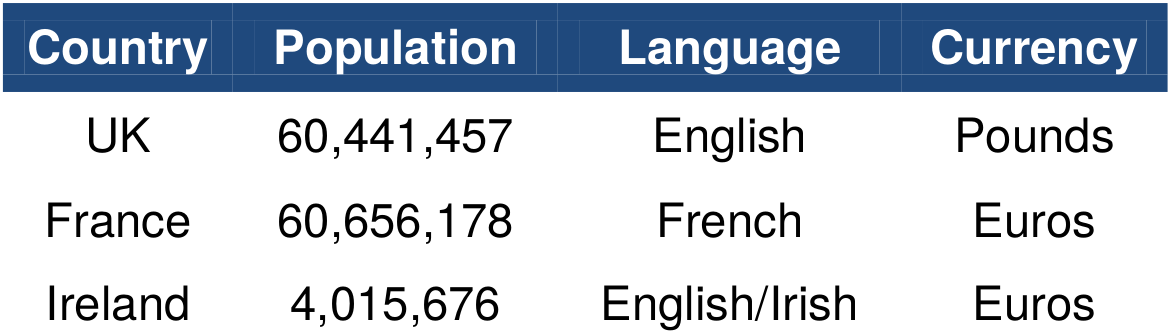
\includegraphics[width=0.9\textwidth]{c9_enzyme_ref_cds.png}
  \end{figure}
\end{frame}

\begin{frame}[fragile]
  \frametitle{引用 | 复杂数据结构}
  \vspace{-0.6em}
\begin{lstlisting}[basicstyle=\small\tt]
my %countries;
my %uk_info = (
    population => 60441457,
    language => 'English',
    currency => 'Pounds',
);
my %france_info = (
    population => 60656178, language => 'French', currency => 'Euros',
);
my %ireland_info = ( ... );

$countries{uk} = \%uk_info;
$countries{france} = \%france_info;
#$countries{ireland} = \%ireland_info;

print "Population of France is ",
    $countries{france}->{population},"\n";
\end{lstlisting}
\end{frame}

\begin{frame}[fragile]
  \frametitle{引用 | 复杂数据结构}
  \vspace{-0.6em}
\begin{lstlisting}[basicstyle=\small\tt]
my %countries = (
    uk => {
        population => 60441457,
        language => 'English',
        currency => 'Pounds',
    },
    france => {
        population => 60656178,
        language => 'French',
        currency => 'Euros',
    },
    ireland => {
        ...
    },
);

print "Population of France is ",
    $countries{france}->{population},"\n";
\end{lstlisting}
\end{frame}

\begin{frame}[fragile]
  \frametitle{引用 | 复杂数据结构}
\begin{lstlisting}[basicstyle=\small\tt]
my %countries;

$countries{uk}     -> {population} = 60441457;
$countries{france} -> {population} = 60656178;
$countries{france} -> {currency}   = 'Euros';

print "Population of France is ",
    $countries{france}->{population},"\n";
\end{lstlisting}
\end{frame}

\begin{frame}[fragile]
  \frametitle{引用 | 复杂数据结构 | 多种方法}
  \begin{block}{Data: country.txt}
  \vspace{-0.5em}
\begin{lstlisting}[basicstyle=\footnotesize\tt,numberstyle=\scriptsize]
|----------+------------+---------------+-----------|
|  Country | Population | Language      | Currency  |
|----------+------------+---------------+-----------|
|  UK      | 60,441,457 | English       | Pounds    |
|  France  | 60,656,178 | French        | Euros     |
|  Ireland | 4,015,676  | English/Irish | Euros     |
|----------+------------+---------------+-----------|
\end{lstlisting}
  \end{block}
  \pause
  \begin{block}{Task}
    Q: Population of France\\
    A: 60,656,178
  \end{block}
\end{frame}

\begin{frame}[fragile]
  \frametitle{引用 | 复杂数据结构 | 多种方法}
  \begin{block}{shell}
\begin{lstlisting}
grep -i -w France country.txt | cut -f2
\end{lstlisting}
  \end{block}
  \pause
  \begin{block}{csvkit}
\begin{lstlisting}
# Method 1
csvsql --query "select Population from country where Country=='France'" country.txt | csvlook
# Method 2
csvgrep -t -c Country -m France country.txt | csvcut -c Population | csvlook
\end{lstlisting}
  \end{block}
\end{frame}

\begin{frame}[fragile]
  \frametitle{引用 | 复杂数据结构 | 多种方法}
  \begin{block}{Perl-hash}
  \vspace{-0.6em}
\begin{lstlisting}[basicstyle=\scriptsize\tt,numberstyle=\scriptsize]
#!/usr/bin/perl
use strict; use warnings;
my $fi = "country.txt";
my ( @header, @fields, %countries);
open my $IN, '<', $fi or die "$0 : failed to open  input file '$fi' : $!\n";
while (<$IN>) {
    chomp;
    if ( $. == 1 ) {
        @header = map { lc } split /\t/;
    }
    else {
        @fields = map { lc } split /\t/;
        for ( my $i = 1 ; $i < @header ; $i++ ) {
            $countries{$fields[0]}->{$header[$i]}=$fields[$i];
        }
    }
}
close $IN or warn "$0: failed to close input file '$fi': $!\n";
print "Population of France is ", $countries{france}->{population}, "\n";
\end{lstlisting}
  \end{block}
\end{frame}

\begin{frame}[fragile]
  \frametitle{引用 | 复杂数据结构 | 多种方法}
  \begin{block}{Perl-Data::Table}
\begin{lstlisting}[basicstyle=\small\tt]
#!/usr/bin/perl

use strict;
use warnings;
use Data::Table;

my $countries = Data::Table::fromFile("country.txt");

print "Population of France is ",
  $countries->
  match_pattern_hash('$_{Country} eq "France"')->
  col('Population'),
  "\n";
\end{lstlisting}
  \end{block}
\end{frame}

\begin{frame}[fragile]
  \frametitle{引用 | 复杂数据结构 | 多种方法}
  \begin{block}{R}
\begin{lstlisting}[language=r]
#!/usr/bin/Rscript

library(readr)
library(dplyr)

countries <- read_tsv("country.txt")
countries %>% 
  filter(Country=="France") %>% 
  select(Population) %>%
  pull()
\end{lstlisting}
  \end{block}
\end{frame}

\begin{frame}[fragile]
  \frametitle{引用 | 复杂数据结构}
  \vspace{-0.8em}
\begin{lstlisting}[basicstyle=\footnotesize\tt,numberstyle=\scriptsize]
my @experiments = (
    {
        sample_id => 1,
        sample_name => 'kidney',
        sample_measures => [12,56,34,65,76],
    },
    {
        sample_id => 4,
        sample_name => 'liver',
        sample_measures => [24,66,12,17,26],
    },
    { ... },
);

foreach my $expt (@experiments) {
    print "The first measure for sample ",
          $expt->{sample_id},
          " (",$expt->{sample_name},") was ",
          $expt->{sample_measures}->[0],"\n";
}
\end{lstlisting}
\end{frame}

\section{模块}
\begin{frame}[fragile]
  \frametitle{模块 | 安装}
  \vspace{-0.6em}
\begin{lstlisting}
# METHOD 1: cpan
#Open cpan shell
sudo cpan #Or
perl -MCPAN -e shell
#Install modules
cpan>install Date::Calc

# METHOD 2: cpanm
#Install cpanm
#perlbrew is an admin-free perl installation management tool
perlbrew install-cpanm
#Install modules
cpanm Bio::Perl

# METHOD 3: manual
\end{lstlisting}
\end{frame}

\begin{frame}[fragile]
  \frametitle{模块 | 使用 | 函数式编程}
\begin{lstlisting}
#!/usr/bin/perl

use warnings;
use strict;

use Date::Calc qw(:all);
#use Date::Calc qw(Days_in_Year Days_in_Month);

print "In Feb 2020 there are ",Days_in_Month(2020,2)," days";
\end{lstlisting}
\end{frame}

\begin{frame}[fragile]
  \frametitle{模块 | 使用 | 面向对象编程}
  \vspace{-0.6em}
  \begin{lstlisting}[basicstyle=\small\tt]
#!/usr/bin/perl

use warnings; use strict;

use LWP::UserAgent;
 
my $ua = LWP::UserAgent->new;
$ua->timeout(10);
$ua->env_proxy;
 
my $response=$ua->get('http://search.cpan.org/');
 
if ($response->is_success) {
    print $response->decoded_content;
}
else {
    die $response->status_line;
}
\end{lstlisting}
\end{frame}

\begin{frame}[fragile]
  \frametitle{模块 | 编写 | 函数式编程}
\begin{lstlisting}
#!/usr/bin/perl

use warnings;
use strict;

package Example::Module;

# Module code goes here

1;
\end{lstlisting}
\end{frame}

\begin{frame}[fragile]
  \frametitle{模块 | 编写 | 函数式编程}
\begin{lstlisting}[basicstyle=\scriptsize\tt,numberstyle=\scriptsize]
#!/usr/bin/perl
use warnings; use strict;

use Exporter;
our @ISA = qw(Exporter);
our @EXPORT_OK = qw(will_be_exported);

sub public {
    # This is designed to be seen, but can only be addressed by using its fully qualified name eg Example::Functional::public()
}
sub _private {
    # This is only for internal use and shouldn't be used from outside the module.
}
sub will_be_exported {
    # This can be exported into the namespace of the calling program
}

1;
\end{lstlisting}
\end{frame}

\begin{frame}[fragile]
  \frametitle{模块 | 编写 | 面向对象编程(1/2)}
\begin{lstlisting}[basicstyle=\footnotesize\tt,numberstyle=\scriptsize]
#!/usr/bin/perl

use warnings;
use strict;

package Example::Object_oriented;

sub new {
    # This creates the refernece which is going to be our object
    my $hashref = {};
    # We then call bless to associate it with this module.
    bless $hashref;
    # Finally we return it so the calling program can start using it.
    return $hashref;
}
\end{lstlisting}
\end{frame}

\begin{frame}[fragile]
  \frametitle{模块 | 编写 | 面向对象编程(2/2)}
  \vspace{-0.8em}
\begin{lstlisting}[firstnumber=16,basicstyle=\footnotesize\tt,numberstyle=\scriptsize]
sub save_value {
    # This subroutine takes a single arguement which it stores in the hash reference. The $object is provided automatically as the first argument to every object oriented subroutine (other than 'new').
    my ($object, $new_value) = @_;
    $object->{value} = $new_value;
}
sub get_value {
    # This subroutine retrieves a value which was previously stored via the save_value subroutine. If there isn't a value to retrieve it returns the undefined value.
    my ($object) = @_;
    if (exists $object->{value}) {return $object->{value};}
    else { return undef; }
}

1;
\end{lstlisting}
\end{frame}

\begin{frame}[fragile]
  \frametitle{模块 | 编写 | 面向对象编程 | 使用}
\begin{lstlisting}
#!/usr/bin/perl

use warnings;
use strict;

use Example::Object_oriented;

my $object = Example::Object_oriented->new();

$object->save_value("Hello");

print "The object says '". $object->get_value() . "'\n";
\end{lstlisting}
\end{frame}

\section{BioPerl}
\begin{frame}[fragile]
  \frametitle{BioPerl}
\begin{lstlisting}[basicstyle=\footnotesize\tt,numberstyle=\scriptsize]
use Bio::SeqIO;

my $string = ">SEQ1\nacgt\n>revseq1\ntgca "; 
my $format = "fasta";

my $stringfh = IO::String->new($string); 
open($stringfh, "<", $string) or die "Could not open string for reading: $!";

my $seqio = Bio::SeqIO-> new(-fh     => $stringfh,
                             -format => $format,
                            );

while( my $seq = $seqio->next_seq ) {
   print $seq->id . ' = ' . $seq->seq() . "\n"; 
}
\end{lstlisting}
\end{frame}

\begin{frame}[fragile]
  \frametitle{BioPerl}
\begin{lstlisting}[basicstyle=\footnotesize\tt,numberstyle=\scriptsize]
use strict; use Bio::SeqIO;
my $input_file = shift;
my $seq_in = Bio::SeqIO->new( -format => 'embl',
                              -file   => $input_file,
                             );
my @seq_array; 
while ( my $seq = $seq_in->next_seq() ) {
   push(@seq_array,$seq);
}
@seq_array = sort { $a->length <=> $b->length } @seq_array;
my $total = 0; 
my $count = 0; 
for my $seq ( @seq_array ) {
   $total += $seq->length;
   $count++;
}
print "Mean length ", $total/$count, " Median ", 
      $seq_array[$count/2]->length, "\n";
\end{lstlisting}
\end{frame}

\begin{frame}[fragile]
  \frametitle{BioPerl}
\begin{lstlisting}[basicstyle=\footnotesize\tt,numberstyle=\scriptsize]
use Bio::SeqIO;

my $usage = "x2y.pl infile informat outfile outformat "; 
my $infile = shift or die $usage; 
my $informat = shift or die $usage; 
my $outfile = shift or die $usage; 
my $outformat = shift or die $usage;

my $seq_in = Bio::SeqIO->new( -file   => "$infile",
                              -format => $informat,
                            );
my $seq_out = Bio::SeqIO->new( -file   => ">$outfile",
                               -format => $outformat,
                             );
while (my $inseq = $seq_in->next_seq) {
   $seq_out->write_seq($inseq);
}
\end{lstlisting}
\end{frame}

\begin{frame}[fragile]
  \frametitle{BioPerl}
  \vspace{-0.6em}
\begin{lstlisting}[basicstyle=\tiny\tt,numberstyle=\tiny]
use Bio::SeqIO;
my $usage = "splitgb.pl infile "; my $infile = shift or die $usage;
my $inseq = Bio::SeqIO->new( -file   => "<$infile", -format => 'Genbank',);
my %outfiles = ( human => {
                         Genbank => Bio::SeqIO->new(
                                                    -file   => '>human.gb',
                                                    -format => 'Genbank',
                                                    ),
                         Fasta   => Bio::SeqIO->new(
                                                    -file   => '>human.fa',
                                                    -format => 'Fasta',
                                                    ),
                         },
                 other => {
                         Genbank => Bio::SeqIO->new(
                                                    -file   => '>other.gb',
                                                    -format => 'Genbank',),
                         Fasta   => Bio::SeqIO->new(
                                                    -file => '>other.fa',
                                                    -format => 'Fasta',),
                         }
               );
while (my $seqin = $inseq->next_seq) {
   if ($seqin->species->binomial =~ m/Homo sapiens/) {
       $outfiles{'human'}->{'Genbank'}->write_seq($seqin);
       $outfiles{'human'}->{'Fasta'}->write_seq($seqin);
   } else {
       $outfiles{'other'}->{'Genbank'}->write_seq($seqin);
       $outfiles{'other'}->{'Fasta'}->write_seq($seqin);
   }
}
\end{lstlisting}
\end{frame}

\begin{frame}[fragile]
  \frametitle{BioPerl}
\begin{lstlisting}[basicstyle=\footnotesize\tt,numberstyle=\scriptsize]
use Bio::DB::GenBank;
use Bio::DB::Query::GenBank;

$query = "Arabidopsis[ORGN] AND topoisomerase[TITL] and 0:3000[SLEN]"; 
$query_obj = Bio::DB::Query::GenBank->new(-db => 'nucleotide', 
                                          -query => $query );

$gb_obj = Bio::DB::GenBank->new;

$stream_obj = $gb_obj->get_Stream_by_query($query_obj);

while ($seq_obj = $stream_obj->next_seq) {
    # do something with the sequence object    
    print $seq_obj->display_id, "\t", $seq_obj->length, "\n";
}
\end{lstlisting}
\end{frame}

\begin{frame}[fragile]
  \frametitle{BioPerl}
  \vspace{-0.8em}
\begin{lstlisting}[basicstyle=\scriptsize\tt,numberstyle=\tiny]
#!/usr/bin/perl
use strict; use warnings;
use Bio::DB::Query::GenBank; use Bio::DB::GenBank;
use Bio::SeqIO;

my $query_string = $ARGV[0];
my $fo_fa=$query_string.".fa"; my $fo_gb=$query_string.".gb";
my $query = Bio::DB::Query::GenBank->new(
    -db => 'nucleotide', -query => $query_string
);
my $gb = Bio::DB::GenBank->new;
my $stream = $gb->get_Stream_by_query($query);

my %outfiles = (
    Fasta => Bio::SeqIO->new( -file => ">$fo_fa", -format => 'Fasta',),
    Genbank => Bio::SeqIO->new( -file => ">$fo_gb", -format => 'Genbank',),
);
while ( my $seq = $stream->next_seq ) {
    $outfiles{'Fasta'}->write_seq($seq);
    $outfiles{'Genbank'}->write_seq($seq);
}
\end{lstlisting}
\end{frame}


\input{snippet/class_tail.tex}
